\begin{enumerate}
    \item \phantom{0}
    \begin{center}
    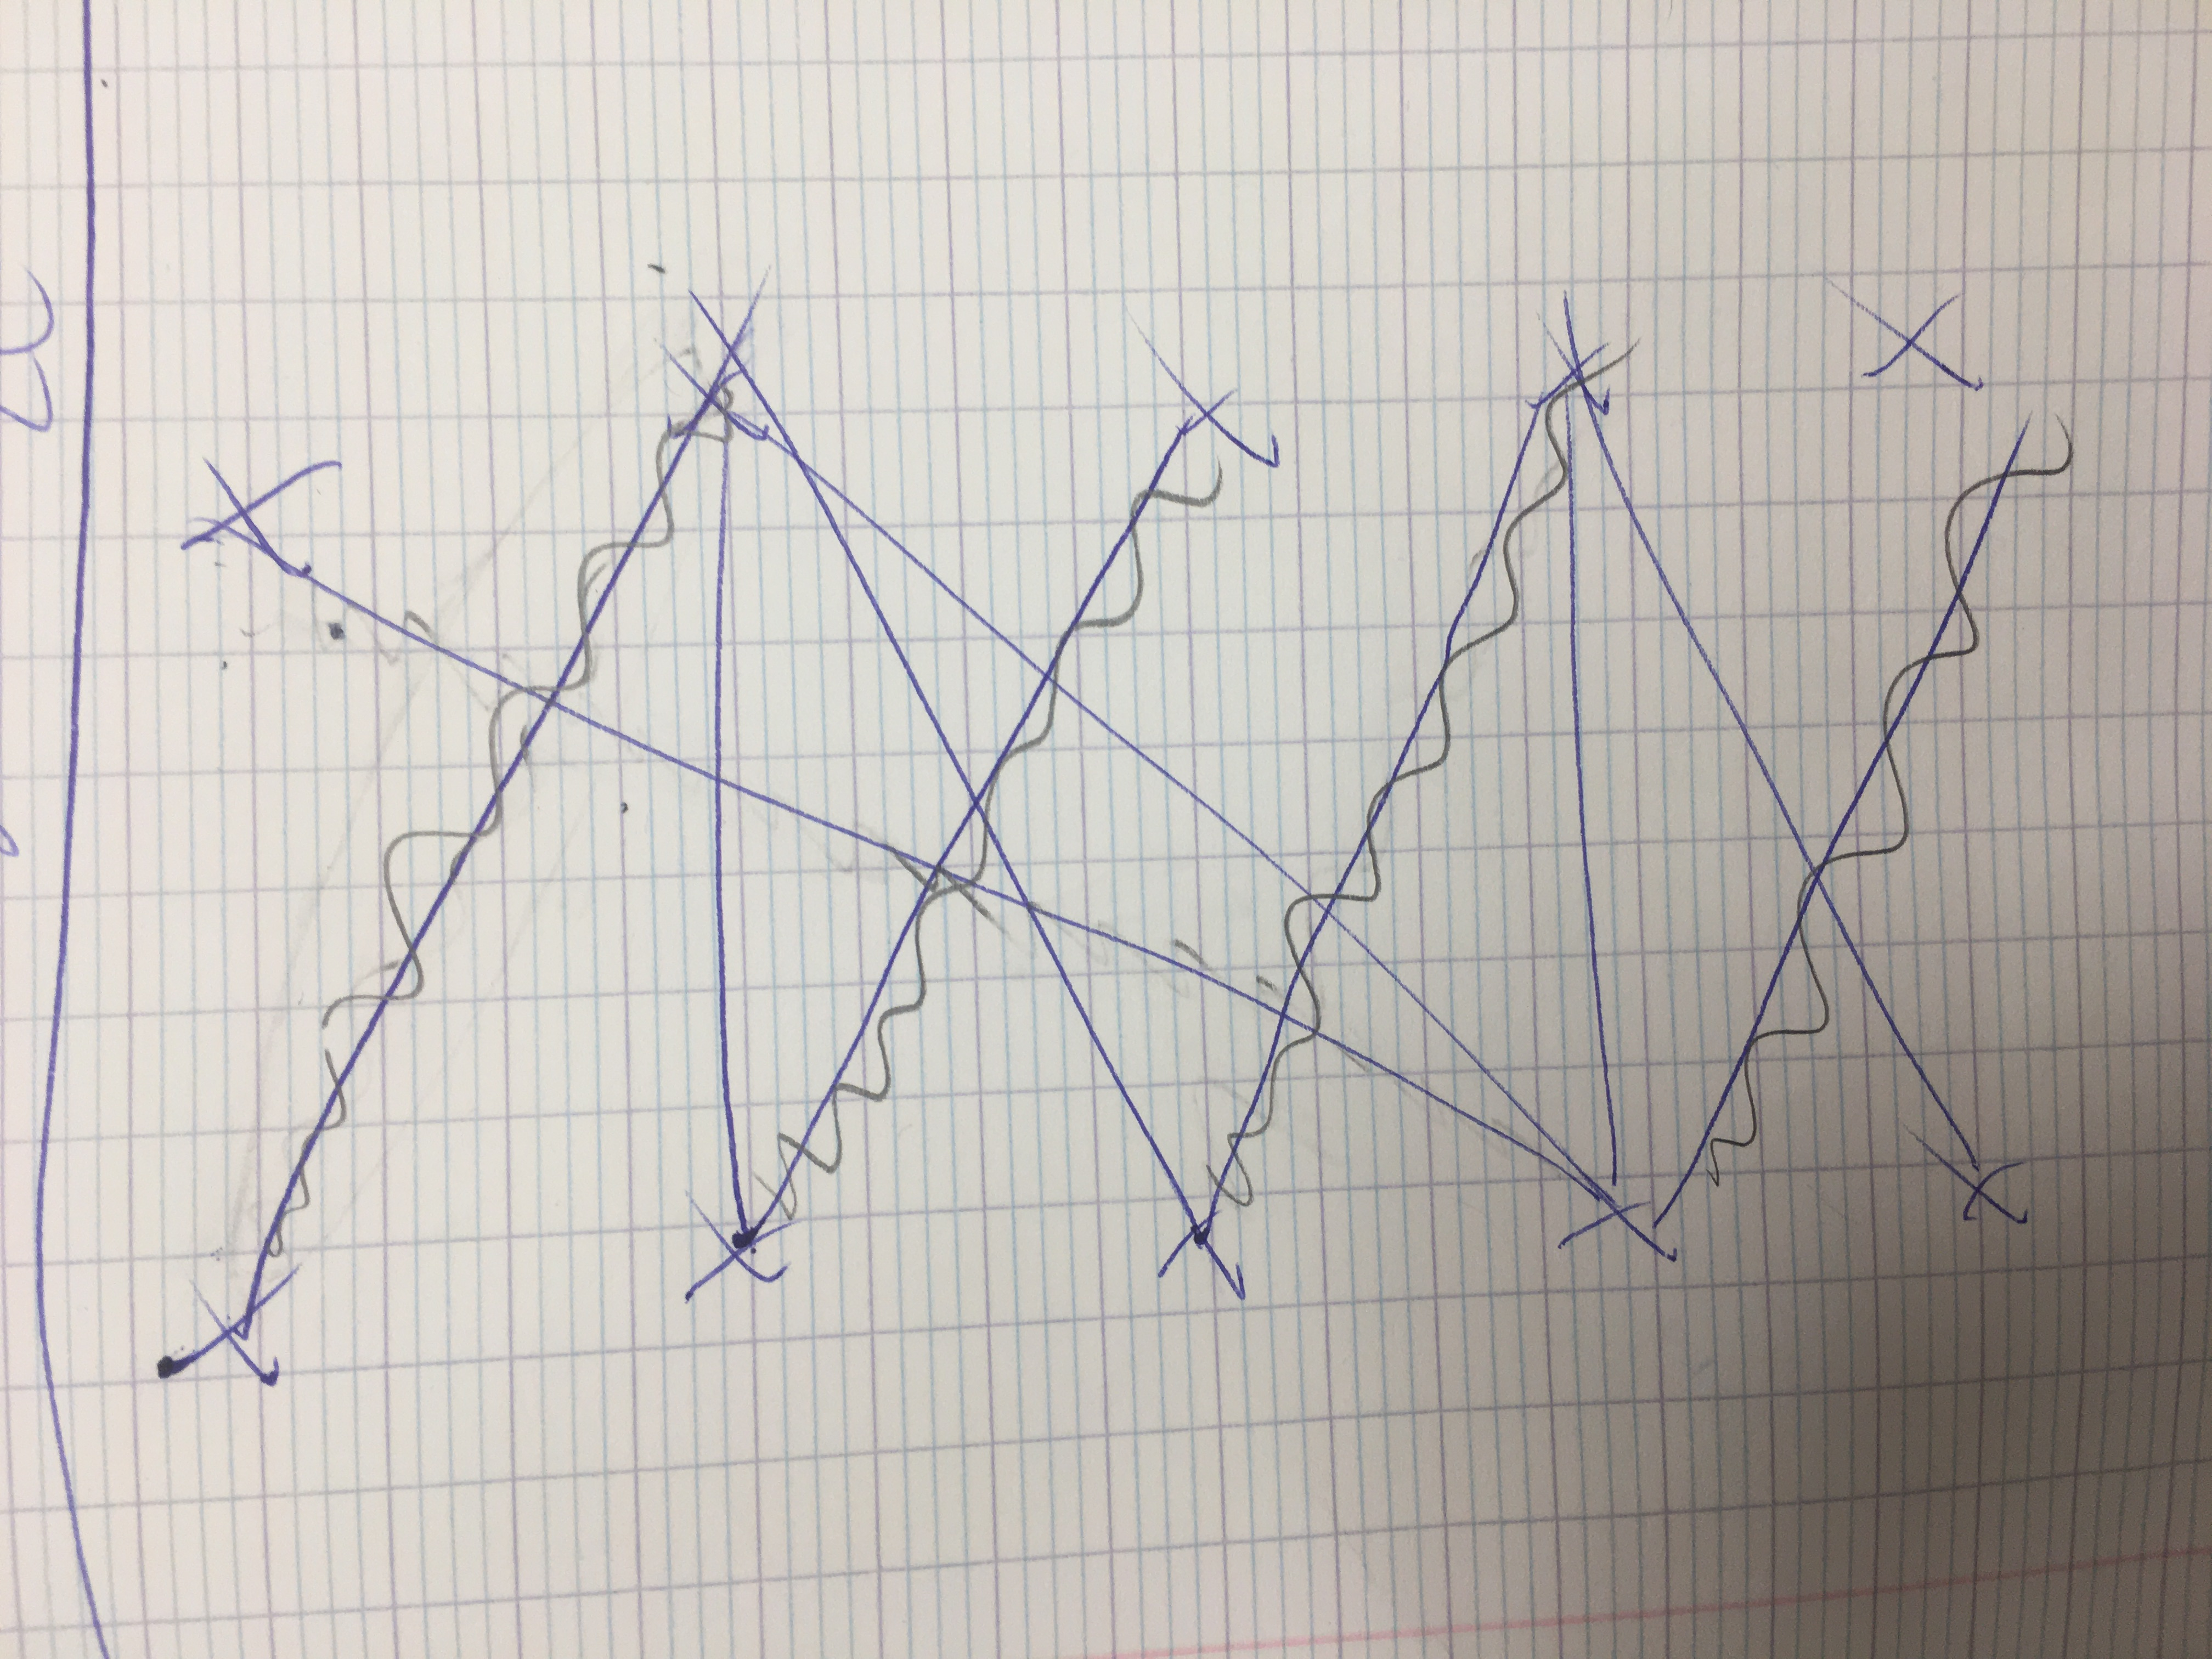
\includegraphics[width=0.6\textwidth]{figures/IMG_1229.jpg}
    \end{center}
    \item On ajoute un puit et une source, qu'on relie respectivement par chacune des deux portions des sommets du graphe (puisqu'il est biparti) puis on définit toutes les capacités comme étant unaires.
    \begin{center}
    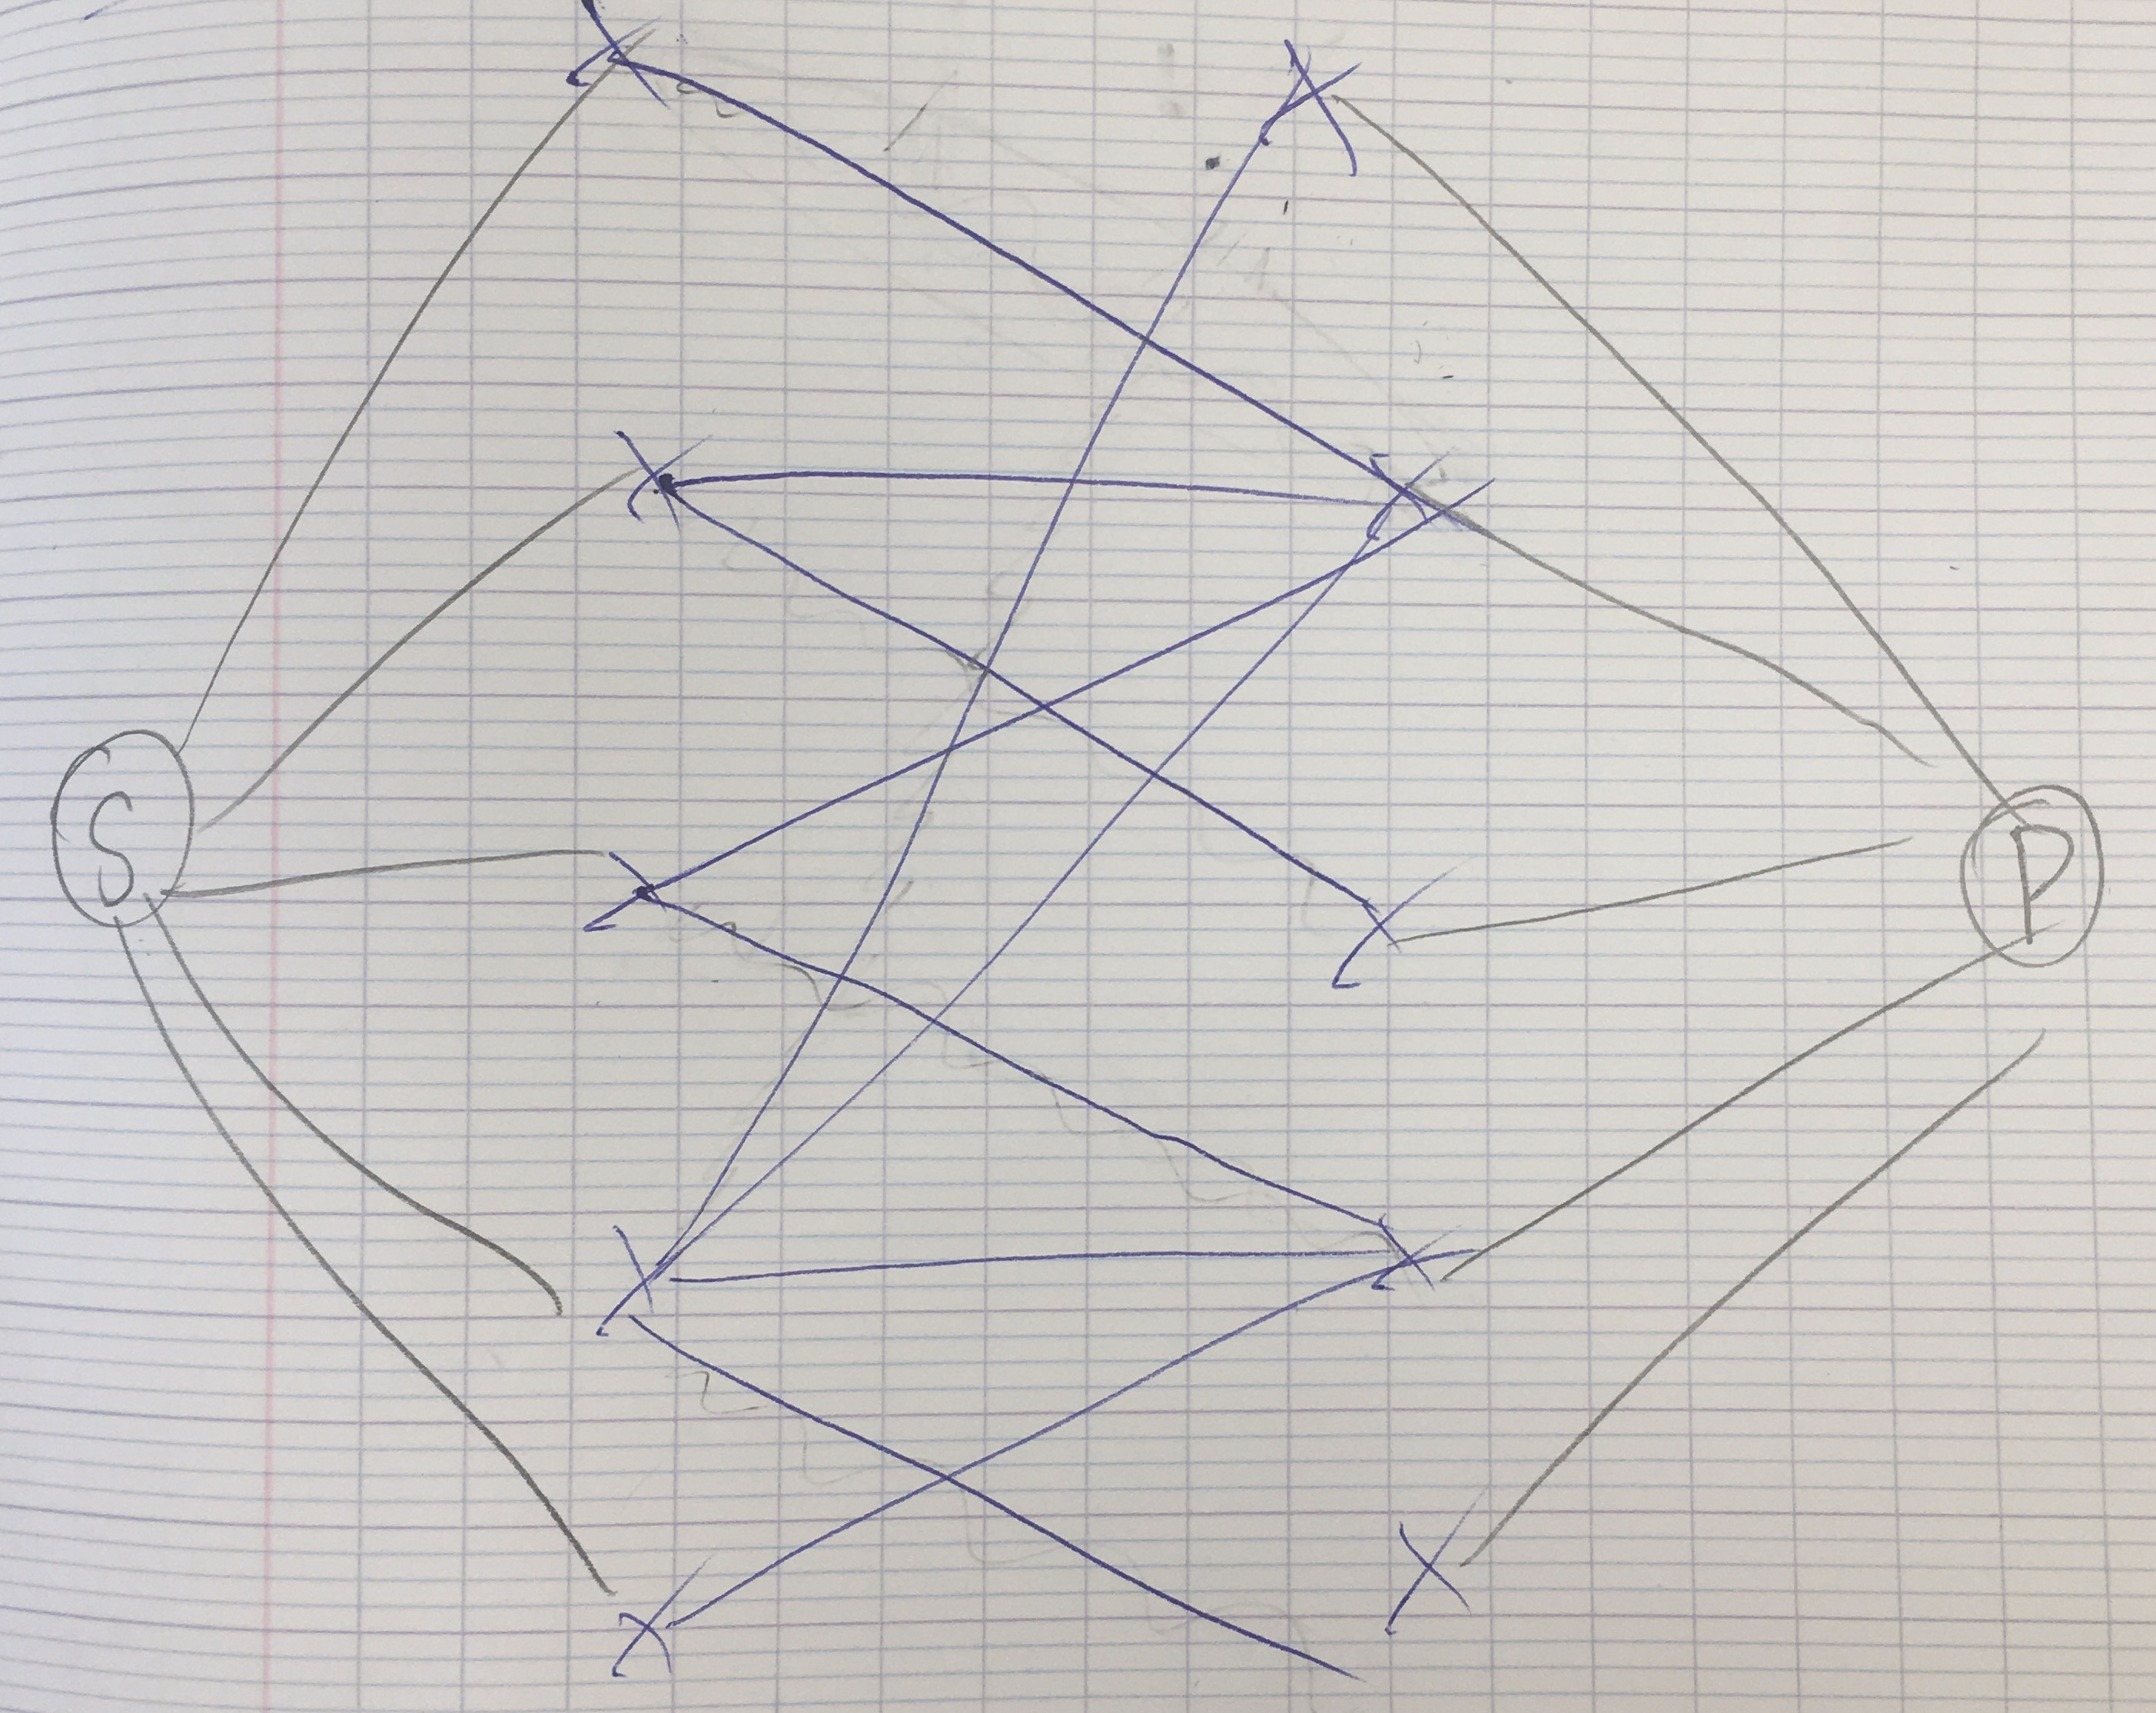
\includegraphics[width=0.75\textwidth]{figures/IMG_1230.jpg}
    \end{center}
    Cette opération se fait en un temps linéaire en le nombre de sommets du graphe. Puis, un flot maximum obtenu est alors un couplage maximum du graphe de départ.

    \item Réciproquement, Il suffit de supprimer du réseau le sommet et le puis, d'omettre les capacités, et de considérer les arêtes du réseau comme des arêtes du graphe de départ. La complexité est linéaire en la somme des degrés du puit et de la source. Un couplage maximum du réseau correspond alors à un flot maximum du graphe de départ.
    \item Il est clair que les fonctions $\varphi$ et $\psi$ ainsi définies sont inverses l'une de l'autre, et que les appliquer successivement à un graphe biparti nous ramène au même graphe biparti, ce qui justifie qu'on obtient une instance du problème initial.
    \item Selon le site de \href{https://dept-info.labri.fr/~baudon/Licence/Algo2/Cours/Cours/AG9.pdf}{Bordeaux-INP}, on peut appliquer l'algorithme de Ford-Fulkerson pour trouver un flot maximum dans un réseau de transport, et ainsi trouver un couplage maximum dans un graphe biparti. La complexité de cet algorithme est $\bigO(m \cdot f)$, où $m$ est le nombre d'arêtes du graphe et $f$ est la valeur du flot maximum. Cependant, il existe des algorithmes plus efficaces pour les graphes bipartis, tels que l'algorithme de Hopcroft-Karp, qui a une complexité de $\bigO(\sqrt{n} \cdot m)$, où $n$ est le nombre de sommets du graphe.
    \item Pour résoudre le problème du flot maximal, on peut utiliser la méthode de \href{https://mitmgmtfaculty.mit.edu/jorlin/?getPage=Max_flows_in_O%28nm%29_time}{James B. Orlin} en un temps $\bigO(\abs{V}\abs{E})$, ce qui cumulé aux coûts de réduction donne une complexité du même ordre de grandeur. C'est moins favorable que de résoudre directement le problème du couplage maximum dans un graphe biparti, qui peut être fait en $\bigO(\sqrt{\abs{V}} \cdot \abs{E})$ avec l'algorithme de Hopcroft-Karp.
\end{enumerate}